\documentclass[10pt]{article}
\usepackage[letterpaper,landscape,margin=0.65in]{geometry}
\usepackage{graphicx}
\usepackage[T1]{fontenc}
\usepackage{hyperref}
\hypersetup{pdftitle={Lean irreducibility of BINSTD degree-eight factors}}
\setlength{\parindent}{0pt}
\setlength{\parskip}{0.48em}
\title{Lean irreducibility of BINSTD degree-eight factors}
\author{Validation audit, 22 October 2026}
\date{}
\begin{document}
\maketitle
\vspace{-2em}

\textbf{Frozen source.} The n=17 BINSTD Stage-1 files list
bitmask polynomials 313 and 471. The parent Lean task binds these
exact coefficient patterns and proves that their product with
$X+1$ is $X^{17}+1$ over $\mathbf F_2$.

\textbf{New theorem.} The two degree-eight polynomials
\[
X^8+X^5+X^4+X^3+1,\qquad
X^8+X^7+X^6+X^4+X^2+X+1
\]
are both irreducible in $(\mathbf Z/2\mathbf Z)[X]$.
The proof identifies their product with $\Phi_{17}$, checks that
2 has multiplicative order 8 modulo 17 and that both factors have
degree 8, then applies Mathlib's cyclotomic factor-degree criterion.
The formal task targets their conjunction. The verification receipt
reports a passing full build, standard axioms only across 625 audited
theorems, and a passing target audit under Lean 4.35.0-rc1.
Independent semantic review remains pending.

\textbf{Boundary.} This does not yet identify the archived field's
Frobenius with the cyclic normal-basis module or classify all
invariant subspaces. A separate open problem names that bridge.
No empirical yield, performance or security claim follows.

\newpage
\begin{center}
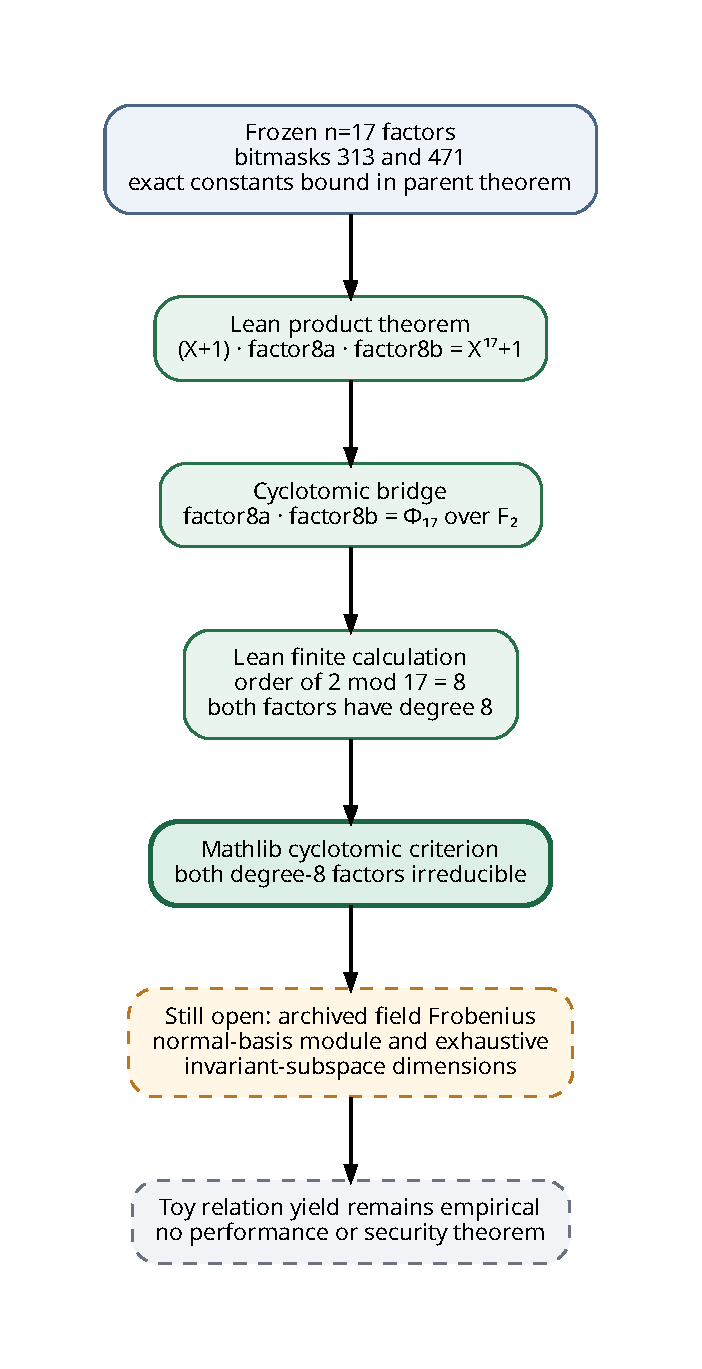
\includegraphics[width=\textwidth,height=0.82\textheight,keepaspectratio]{irreducibility-figure.pdf}
\end{center}
\end{document}
